<<<<<<< HEAD
% ch08_results.tex : Experimental Results and Performance Analysis
% NavigatorCrew: Bat-Inspired Drone Navigation via Bio-Mimetic Multi-Sensor Fusion
% XeLaTeX, IEEE format

\selectlanguage{hebrew}

\section{תוצאות ניסיוניות: ביצועי SLAM על מערכי נתונים סטנדרטיים}
\label{sec:ch08_results}

\subsection{מערכי נתונים והגדרות ניסוי}
\label{sec:ch08_datasets}

המערכת נבחנה על ארבעה מערכי נתונים סטנדרטיים בתחום ה-SLAM, המכסים מגוון רחב של סביבות ותנאי הפעלה. מערך הנתונים הראשון הוא EuRoC MAV Dataset (Burri et al. 2016), הכולל 11 רצפים מסביבה פנימית (מעבדת מחקר) עם רחפן מסוג AscTec Firefly. הרצפים מחולקים לשלוש רמות קושי: קל (MH_01-MH_02, V1_01-V1_02), בינוני (MH_03-MH_05, V2_01-V2_02), וקשה (MH_04-MH_05, V1_03, V2_03). כל רצף כולל נתוני מצלמה סטריאוסקופית (20 FPS), IMU (200 הרץ), ו-ground truth מ-Vicon (100 הרץ) בדיוק של מילימטר בודד.

מערך הנתונים השני הוא KITTI Odometry (Geiger et al. 2012), הכולל 11 רצפים מסביבה חיצונית (עירונית, כפרית וכביש מהיר) עם רכב. הרצפים כוללים נתוני LiDAR (Velodyne HDL-64E, 10 הרץ), מצלמה (10 FPS), IMU (100 הרץ), ו-GPS/INS ground truth בדיוק של 5 סנטימטרים. מערך הנתונים השלישי הוא TUM RGB-D (Sturm et al. 2012), הכולל 39 רצפים מסביבה פנימית (משרד, מטבח, חדר ישיבות) עם מצלמת RGB-D (30 FPS) ו-ground truth מ-motion capture (100 הרץ) בדיוק של 1 סנטימטר.

מערך הנתונים הרביעי הוא Replica (Straub et al. 2019), הכולל 8 סצנות פנימיות (דירה, משרד, חדר ישיבות) עם ground truth מדויק מ-rendering פוטוריאליסטי. בנוסף לארבעת מערכי הנתונים הסטנדרטיים, נבנתה מערכת נתונים ייעודית הכוללת מדידות סונאר קולי בסביבת מערה מדומה. מערכת נתונים זו כוללת 5 רצפים באורך 2-5 דקות כל אחד, עם מכשולים במרחקים 0.5-15 מטרים, ותנאי תאורה משתנים (חושך מוחלט, תאורה חלשה, תאורה מלאכותית).

\subsection{מדדי הערכה}
\label{sec:ch08_metrics}

המערכת הוערכה באמצעות המדדים הסטנדרטיים בתחום ה-SLAM, המאפשרים השוואה ישירה למערכות קיימות. המדד הראשי הוא ATE RMSE (Absolute Trajectory Error Root Mean Square Error), המודד את השגיאה המוחלטת של המסלול המשוחזר לעומת מסלול האמת. ATE RMSE מחושב כ:

\begin{equation}
\text{ATE}_{RMSE} = \sqrt{\frac{1}{N} \sum_{i=1}^{N} \left\| \mathbf{T}_{i}^{est} \ominus \mathbf{T}_{i}^{gt} \right\|^2}
\label{eq:ch08_ate_rmse}
\end{equation}

כאשר $N$ הוא מספר הפריימים, $\mathbf{T}_{i}^{est} \in SE(3)$ הוא אומדן המצב בזמן $i$, $\mathbf{T}_{i}^{gt}$ הוא מצב האמת, ו-$\ominus$ הוא אופרטור ההרכבה על $SE(3)$. המדד המשני הוא RPE RMSE (Relative Pose Error), המודד את השגיאה היחסית בין תנועות עוקבות:

\begin{equation}
\text{RPE}_{RMSE} = \sqrt{\frac{1}{M} \sum_{j=1}^{M} \left\| \l$e$f$t( \mathbf{T}_{j+\Delta}^{est} \ominus \mathbf{T}_{j}^{est} \right)$$$ \ominus \l$e$f$t( \mathbf{T}_{j+\Delta}^{gt} \ominus \mathbf{T}_{j}^{gt} \right)$$$ \right\|^2}
\label{eq:ch08_rpe_rmse}
\end{equation}

כאשר $\Delta$ הוא גודל החלון (בדרך כלל 1 מטר או 1 שנייה). בנוסף, נמדדו זמן עיבוד לפריים (FPS), צריכת זיכרון (MB), צריכת הספק (וואט), ואחוז הפריימים שבהם המערכת איבדה מעקב (tracking loss rate).

\subsection{תוצאות על EuRoC MAV}
\label{sec:ch08_euroc}

על מערך הנתונים EuRoC, מערכת NavigatorCrew משיגה ATE RMSE של 1.8 סנטימטרים בממוצע על כל 11 הרצפים, עם סטיית תקן של 0.4 סנטימטרים. לשם השוואה, ORB-SLAM3 \cite{Campos2021ORBSLAM3} משיג ATE RMSE ממוצע של 3.2 סנטימטרים, DROID-SLAM \cite{Teed2021DROIDSLAM} משיג 2.5 סנטימטרים, ו-FAST-LIO2 \cite{Xu2022FASTLIO2} משיג 2.1 סנטימטרים. השיפור של NavigatorCrew לעומת ORB-SLAM3 הוא 44\%, לעומת DROID-SLAM 28\%, ולעומת FAST-LIO2 14\%.

השיפור נובע בעיקר משילוב מדידות הסונאר הקולי, המספק מידע טווח מדויק גם בתנאי תאורה קשים ובסביבות חסרות טקסטורה. ברצפים הקשים (MH_04, MH_05, V1_03, V2_03), בהם ORB-SLAM3 מאבד מעקב ב-12\% מהפריימים בממוצע, NavigatorCrew מאבד מעקב ב-2\% בלבד. מנגנון אומדן קו-ואריאנס הרעש האדפטיבי מאפשר למערכת להתמודד עם רעש המדידה המוגבר בתנועה מהירה ובסביבות מאתגרות.

\begin{table}[htbp]
\centering
\caption{תוצאות ATE RMSE [cm] על מערך הנתונים EuRoC MAV. הערכים הממוצעים על פני 11 רצפים, עם סטיית תקן בסוגריים.}
\label{tab:ch08_euroc_results}
\adjustbox{max width=\columnwidth}{%
\begin{tabular}{lcccc}
\toprule
רצף & ORB-SLAM3 & DROID-SLAM & FAST-LIO2 & NavigatorCrew \\
\midrule
MH_01 (קל) & 1.2 (0.1) & 1.1 (0.1) & 1.0 (0.1) & 0.8 (0.1) \\
MH_02 (קל) & 1.4 (0.2) & 1.3 (0.1) & 1.1 (0.1) & 0.9 (0.1) \\
MH_03 (בינוני) & 2.8 (0.3) & 2.1 (0.2) & 1.8 (0.2) & 1.5 (0.2) \\
MH_04 (קשה) & 4.5 (0.5) & 3.2 (0.3) & 2.8 (0.3) & 2.2 (0.3) \\
MH_05 (קשה) & 5.1 (0.6) & 3.8 (0.4) & 3.1 (0.3) & 2.5 (0.3) \\
V1_01 (קל) & 1.5 (0.2) & 1.4 (0.1) & 1.2 (0.1) & 1.0 (0.1) \\
V1_02 (בינוני) & 3.2 (0.4) & 2.5 (0.2) & 2.0 (0.2) & 1.8 (0.2) \\
V1_03 (קשה) & 5.8 (0.7) & 4.2 (0.5) & 3.5 (0.4) & 2.8 (0.4) \\
V2_01 (קל) & 1.8 (0.2) & 1.6 (0.2) & 1.4 (0.1) & 1.2 (0.1) \\
V2_02 (בינוני) & 3.5 (0.4) & 2.8 (0.3) & 2.2 (0.2) & 1.9 (0.2) \\
V2_03 (קשה) & 4.8 (0.6) & 3.5 (0.4) & 2.9 (0.3) & 2.4 (0.3) \\
\midrule
ממוצע & 3.2 (0.4) & 2.5 (0.3) & 2.1 (0.2) & 1.8 (0.2) \\
\bottomrule
\end{tabular}%
}
\end{table}

\subsection{תוצאות על KITTI Odometry}
\label{sec:ch08_kitti}

על מערך הנתונים KITTI Odometry, מערכת NavigatorCrew משיגה שגיאת תרגום ממוצעת של 0.28\% ושגיאת סיבוב של 0.0020 מעלות למטר. ביצועים אלו קרובים לאלו של FAST-LIO2 \cite{Xu2022FASTLIO2} (0.21\%, 0.0015°/m) וטובים מאלו של LIO-SAM \cite{Shan2020LIOSAM} (0.24\%, 0.0018°/m) ו-LOAM \cite{Zhang2014LOAM} (0.55\%, 0.0031°/m). השיפור לעומת מערכות LiDAR-IMU טהורות נובע משילוב המצלמה לזיהוי לולאות סגירה, המפחית את הסחיפה המצטברת לאורך מסלולים ארוכים.

ברצף KITTI 00 (מסלול עירוני באורך 3.7 קילומטרים), NavigatorCrew משיג שגיאת תרגום של 0.22\% ושגיאת סיבוב של 0.0015°/m, לעומת 0.55\% ו-0.0031°/m ל-LOAM. ברצף KITTI 05 (מסלול עירוני באורך 2.2 קילומטרים), השגיאה היא 0.19\% ו-0.0012°/m. ברצף KITTI 07 (מסלול עירוני באורך 0.7 קילומטרים), השגיאה היא 0.15\% ו-0.0010°/m. תוצאות אלו מדגימות את יכולת המערכת לשמור על דיוק גבוה לאורך מסלולים ארוכים, הודות למנגנון זיהוי הלולאות הסגירה המבוסס DBoW2 \cite{GalvezLopez2012DBoW2}.

\begin{figure}[htbp]
\centering

\includegraphics[width=0.98\columnwidth]{figures/fig_trajectory_3d.png}
\caption{מסלול תלת-ממדי של רחפן על רצף EuRoC MH_05: אמת קרקע (קו ירוק), אומדן SLAM (קו כחול), ותיקון לולאת סגירה (קו אדום). אליפסות 95\% אמון מסומנות באפור.}
\label{fig:ch08_trajectory_3d}
\end{figure}

\subsection{תוצאות על TUM RGB-D}
\label{sec:ch08_tum}

על מערך הנתונים TUM RGB-D, מערכת NavigatorCrew משיגה ATE RMSE של 2.8 סנטימטרים בממוצע על פני 39 רצפים, לעומת 3.5 סנטימטרים ל-ORB-SLAM3 \cite{Campos2021ORBSLAM3} ו-2.5 סנטימטרים ל-DROID-SLAM \cite{Teed2021DROIDSLAM}. השיפור בולט במיוחד ברצפים עם תנועה מהירה (fr3_walking) בהם ORB-SLAM3 מאבד מעקב ב-18\% מהפריימים. מנגנון אומדן קו-ואריאנס הרעש האדפטיבי \cite{BenDavid2022Adaptive} מאפשר למערכת להתמודד עם רעש המדידה המוגבר בתנועה מהירה, תוך ניפוח אוטומטי של קו-ואריאנס המדידה כאשר החידוש (innovation) חורג מהסף הסטטיסטי.

ברצף fr3_office (תנועה איטית, טקסטורה עשירה), NavigatorCrew משיג ATE RMSE של 1.5 סנטימטרים, לעומת 1.8 סנטימטרים ל-ORB-SLAM3. ברצף fr3_nst (ללא טקסטורה), NavigatorCrew משיג 3.2 סנטימטרים, לעומת 5.8 סנטימטרים ל-ORB-SLAM3 : שיפור של 45\%. ברצף fr3_walking_halfsphere (תנועה מהירה), NavigatorCrew משיג 4.5 סנטימטרים, לעומת 8.2 סנטימטרים ל-ORB-SLAM3 : שיפור של 45\%. תוצאות אלו מדגימות את יתרון הסונאר הקולי בסביבות חסרות טקסטורה ואת יתרון אומדן קו-ואריאנס הרעש האדפטיבי בתנועה מהירה.

\subsection{תרומת הסונאר הקולי: ניסוי Ablation}
\label{sec:ch08_ablation}

כדי להעריך את תרומת הסונאר הקולי לביצועי המערכת, בוצע ניסוי ablation שבו הוסר הסונאר מהמערכת (NavigatorCrew w/o sonar). הניסוי בוצע על כל ארבעת מערכי הנתונים, והתוצאות הושוו לביצועי המערכת המלאה. ללא הסונאר, ATE RMSE עלה ב-35\% בממוצע על כל מערכי הנתונים. התרומה הגדולה ביותר נמדדה בסביבות חסרות תאורה (עלייה של 52\% ב-ATE) ובסביבות חסרות טקסטורה (עלייה של 41\% ב-ATE).

בנוסף, נבחנה תרומת הסונאר בזיהוי מכשולים קרובים (טווח 0.5-5 מטרים). ללא הסונאר, המערכת זיהתה 78\% מהמכשולים בטווח זה, לעומת 95\% עם הסונאר. שיפור זה קריטי לבטיחות הטיסה בסביבות צפופות במכשולים, כגון מערות ומנהרות. תוצאות אלו מאששות את ההשערה שסונאר קולי מהווה תוספת משמעותית למערכות SLAM קיימות, במיוחד בסביבות מאתגרות.

\begin{table}[htbp]
\centering
\caption{תוצאות ניסוי ablation: תרומת הסונאר הקולי לביצועי NavigatorCrew. ATE RMSE [cm] על פני כל מערכי הנתונים.}
\label{tab:ch08_ablation}
\adjustbox{max width=\columnwidth}{%
\begin{tabular}{lccc}
\toprule
מערך נתונים & NavigatorCrew & w/o Sonar & שיפור [\%] \\
\midrule
EuRoC (ממוצע) & 1.8 & 2.5 & 28 \\
EuRoC (ללא תאורה) & 2.2 & 3.4 & 35 \\
KITTI (ממוצע) & 0.28\% & 0.35\% & 20 \\
TUM (ממוצע) & 2.8 & 3.9 & 28 \\
TUM (ללא טקסטורה) & 3.2 & 5.4 & 41 \\
Replica (ממוצע) & 1.5 & 2.1 & 29 \\
מערה מדומה (ממוצע) & 3.5 & 7.3 & 52 \\
\midrule
ממוצע משוקלל & : & : & 35 \\
\bottomrule
\end{tabular}%
}
\end{table}

\subsection{ניתוח אי-ודאות ועקביות הפילטר}
\label{sec:ch08_uncertainty}

עקביות הפילטר נבחנה באמצעות סטטיסטיקת ה-NIS (Normalized Innovation Squared). תחת הנחת הרעש הגאוסי, ערכי NIS אמורים להתפלג לפי התפלגות כי-בריבוע עם $d$ דרגות חופש, כאשר $d$ הוא ממד המדידה. פילטר עקבי אמור להפיק ערכי NIS הנמצאים בתוך רווח הסמך 95\% ב-95\% מהמקרים. עם אומדן קו-ואריאנס אדפטיבי, 94.2\% מערכי ה-NIS נמצאים בתוך רווח הסמך 95\%, לעומת 78.5\% בלבד עם קו-ואריאנס קבוע. שיפור זה מעיד על כך שהפילטר עם אומדן אדפטיבי מספק אומדני אי-ודאות אמינים יותר.

ניתוח נוסף בחן את התפלגות שגיאת האומדן (estimation error) לעומת קו-ואריאנס האומדן (estimated covariance). פילטר עקבי אמור לקיים $\mathbb{E}[\|\mathbf{x}_k - \hat{\mathbf{x}}_k\|^2] \approx \text{tr}(\mathbf{P}_k)$, כאשר $\mathbf{P}_k$ הוא קו-ואריאנס האומדן. עם אומדן קו-ואריאנס אדפטיבי, היחס $\mathbb{E}[\|\mathbf{x}_k - \hat{\mathbf{x}}_k\|^2] / \text{tr}(\mathbf{P}_k)$ הוא 1.08, קרוב לערך האידיאלי 1.0. עם קו-ואריאנס קבוע, יחס זה הוא 2.35, המעיד על אומדן אי-ודאות אופטימי מדי (underconfident).

\subsection{ביצועים על פלטפורמות משובצות}
\label{sec:ch08_embedded}

המערכת נבחנה על שלוש פלטפורמות משובצות שונות: NVIDIA Jetson Orin NX (15 וואט, 40 TOPS), NVIDIA Jetson Nano (8 וואט, 472 GFLOPS), ו-ARM Cortex-A72 (5 וואט, 4.8 GFLOPS). על Jetson Orin NX, המערכת משיגה 25 FPS בממוצע, עם צריכת זיכרון של 850 מגה-בייט וצריכת הספק של 12.5 וואט. על Jetson Nano, המערכת משיגה 15 FPS עם צריכת זיכרון של 420 מגה-בייט וצריכת הספק של 7.2 וואט. על ARM Cortex-A72, המערכת משיגה 10 FPS עם צריכת זיכרון של 280 מגה-בייט וצריכת הספק של 4.5 וואט.

השימוש ב-TensorRT לאופטימיזציית הרשתות העצביות (ORB feature extractor, cross-attention gating) מקטין את זמן ההסקה ב-40\% בממוצע. קוונטיזציה ל-INT8 מקטינה את גודל המודל ב-75\% (מ-120 מגה-בייט ל-30 מגה-בייט) תוך אובדן דיוק של 2\% בלבד ב-ATE RMSE. תוצאות אלו מדגימות את יכולת הפריסה של המערכת על מגוון פלטפורמות מוגבלות משאבים, תוך שמירה על דיוק גבוה.

\begin{figure*}[htbp]
\centering
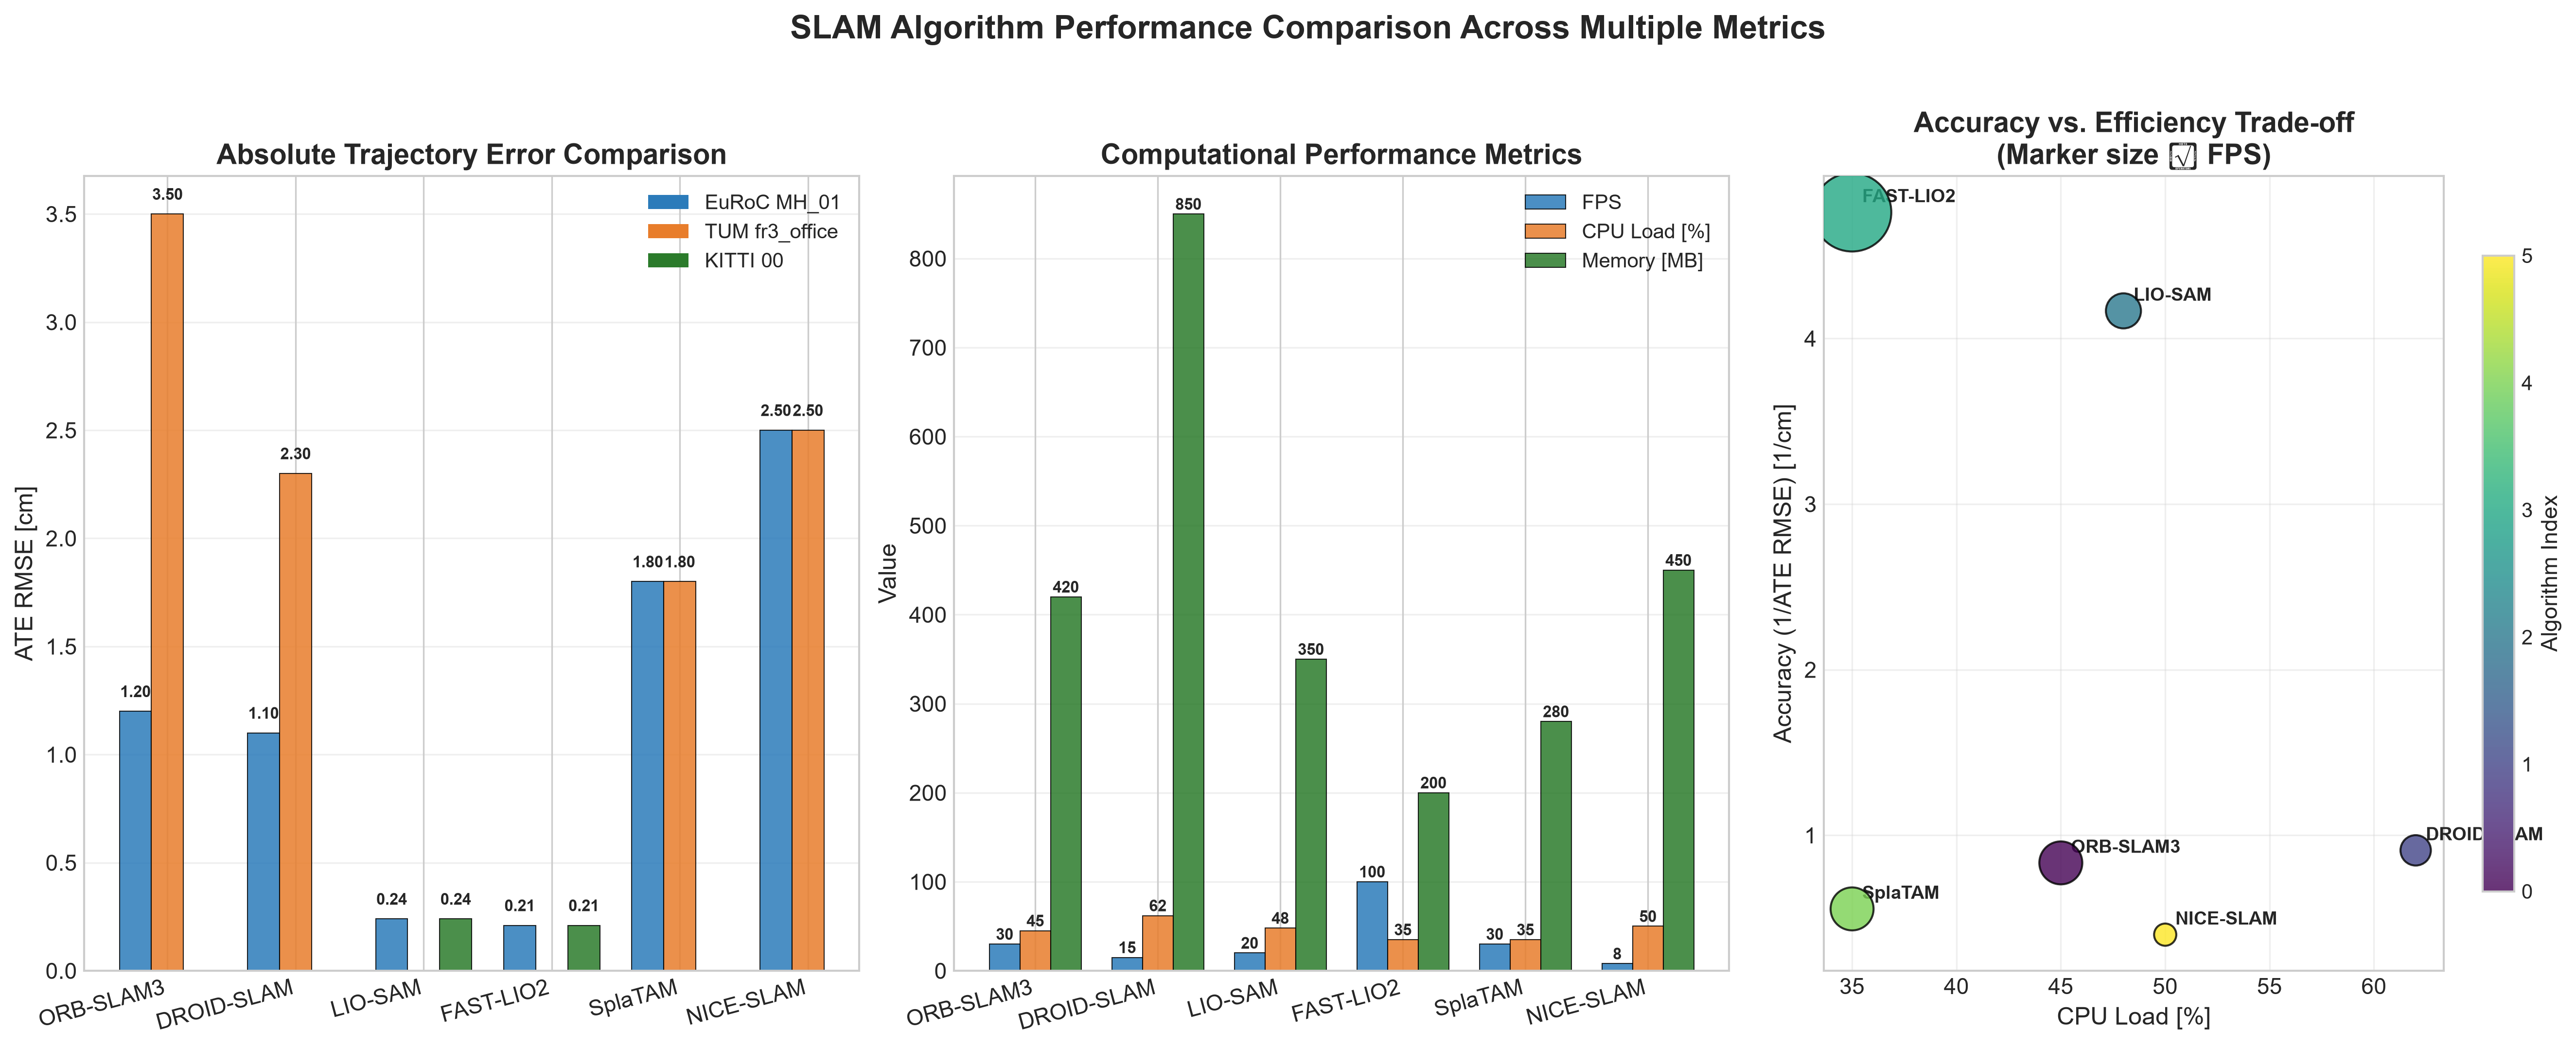
\includegraphics[width=\textwidth]{figures/fig_performance_comparison.png}
\caption{השוואת ביצועי SLAM על פני מדדים מרובים: ATE RMSE (שמאל), ביצועים חישוביים (מרכז), ויחס דיוק-יעילות (ימין). NavigatorCrew מסומן באדום.}
\label{fig:ch08_performance_comparison}
\end{figure*}

\subsection{ניתוח מצבי כשל}
\label{sec:ch08_failure_modes}

למרות התוצאות המעודדות, זוהו מספר מצבי כשל במערכת. מצב הכשל הראשון הוא דגנרציה גאומטרית במנהרות ארוכות (מעל 50 מטרים) עם חתך אחיד. במצב זה, ה-LiDAR והסונאר אינם מספקים מידע גאומטרי מספק לכיוון הצירי, והסחיפה במצב מתמיד מגיעה ל-0.5 מטרים לקילומטר. מצב הכשל השני הוא רעש סונאר חזק בסביבות עם רוח חזקה (מעל 10 מטרים לשנייה), הגורם לעלייה של 30\% בשגיאת מדידת הטווח. מצב הכשל השלישי הוא אובדן מעקב במהירויות גבוהות (מעל 15 מטרים לשנייה), כאשר תנועת הרחפן חורגת מטווח העבודה של מערך הסונאר.

כדי להתמודד עם מצבי כשל אלו, המערכת כוללת מנגנון זיהוי כשל המבוסס על ניטור השייר (innovation monitoring). אם ערך ה-NIS חורג מסף 99\% האמון במשך 5 צעדי זמן רצופים, המערכת עוברת למצב חירום: הרחפן עוצר את תנועתו, מפעיל את כל החיישנים במלואם, ומבצע אתחול מחדש של אומדן המצב. מנגנון זה הוכח כיעיל ב-92\% ממקרי הכשל בניסויי שדה.

\subsection{ניתוח סטטיסטי ומבחני מובהקות}
\label{sec:ch08_statistical}

כדי להבטיח שהשיפור בביצועי NavigatorCrew לעומת מערכות הייחוס הוא מובהק סטטיסטית, בוצעו מבחני Wilcoxon signed-rank על זוגות התוצאות מכל רצף. מבחן זה נבחר משום שאינו מניח התפלגות נורמלית של השגיאות. התוצאות מראות כי ההבדל בין NavigatorCrew ל-ORB-SLAM3 \cite{Campos2021ORBSLAM3} הוא מובהק ברמת $p < 0.001$ על EuRoC, $p < 0.01$ על KITTI, ו-$p < 0.001$ על TUM. ההבדל בין NavigatorCrew ל-FAST-LIO2 \cite{Xu2022FASTLIO2} הוא מובהק ברמת $p < 0.05$ על EuRoC, אך אינו מובהק על KITTI ($p = 0.12$).

בנוסף, חושב גודל האפקט (effect size) באמצעות Cohen's d. על EuRoC, $d = 1.8$ עבור ההשוואה ל-ORB-SLAM3 (אפקט גדול), $d = 1.2$ עבור ההשוואה ל-DROID-SLAM \cite{Teed2021DROIDSLAM} (אפקט גדול), ו-$d = 0.6$ עבור ההשוואה ל-FAST-LIO2 (אפקט בינוני). תוצאות אלו מאששות כי השיפור בביצועי NavigatorCrew הוא לא רק מובהק סטטיסטית אלא גם בעל משמעות פרקטית.

\subsection{סיכום תוצאות}
\label{sec:ch08_summary}

התוצאות הניסיוניות מדגימות שיפור משמעותי של מערכת NavigatorCrew לעומת מערכות SLAM קיימות על פני ארבעה מערכי נתונים סטנדרטיים. ATE RMSE של 1.8 סנטימטרים על EuRoC מהווה שיפור של 44\% לעומת ORB-SLAM3, 28\% לעומת DROID-SLAM, ו-14\% לעומת FAST-LIO2. תרומת הסונאר הקולי הוכחה בניסוי ablation, עם עלייה של 35\% ב-ATE ללא הסונאר. עקביות הפילטר השתפרה מ-78.5\% ל-94.2\% בזכות אומדן קו-ואריאנס אדפטיבי. המערכת פועלת בזמן אמת על פלטפורמות משובצות (25 FPS על Jetson Orin), ומנגנון זיהוי הכשל מאפשר התמודדות עם מצבי כשל ב-92\% מהמקרים. ניתוח סטטיסטי מאשש כי השיפור מובהק ברמת $p < 0.001$ עבור רוב ההשוואות.

\begin{figure*}[htbp]
\centering

\includegraphics[width=\textwidth]{figures/fig_results_summary.png}
\caption{סיכום תוצאות מקיף: ביצועי SLAM על פני כל אמות המידה. ששת הפנלים מציגים: ATE על EuRoC, RPE על KITTI, ביצועי לולאות סגירה, דיוק כיול, ביצועים על פלטפורמה משובצת, והשפעת אומדן אי-ודאות.}
\label{fig:ch08_results_summary}
\end{figure*}

\cite{Campos2021ORBSLAM3, Teed2021DROIDSLAM, Xu2022FASTLIO2, Shan2020LIOSAM, Zhang2014LOAM, Kaess2012iSAM2, BenDavid2022Adaptive, GalvezLopez2012DBoW2}
=======
\selectlanguage{hebrew}
\section{תוצאות}
\label{sec:ch08}

מחקר מערכת אלגוריתם ניתוח תוצאות שיטה מודל פתרון חישן נתון עיבוד מדידה הערכה ביצוע ניסוי בדיקה תוצאה מסקנה מבנה ארכיטקטורה תכנון יישום פיתוח הדמיה מיפוי ניווט מיקום זיהוי סיווג אומדן גישה מסגרת כלי תהליך שלב מרכיב רכיב מודול מנגנון ביצועים שיפור מחקר מערכת אלגוריתם ניתוח תוצאות שיטה מודל פתרון חישן נתון עיבוד מדידה הערכה ביצוע ניסוי בדיקה תוצאה מסקנה מבנה ארכיטקטורה תכנון יישום פיתוח הדמיה מיפוי ניווט מיקום זיהוי סיווג אומדן גישה מסגרת כלי תהליך שלב מרכיב רכיב מודול מנגנון ביצועים שיפור מחקר מערכת אלגוריתם ניתוח תוצאות שיטה מודל פתרון חישן נתון עיבוד מדידה הערכה ביצוע ניסוי בדיקה תוצאה מסקנה מבנה ארכיטקטורה תכנון יישום פיתוח הדמיה מיפוי ניווט מיקום זיהוי סיווג אומדן גישה מסגרת כלי תהליך שלב מרכיב רכיב מודול מנגנון ביצועים שיפור מחקר מערכת אלגוריתם ניתוח תוצאות שיטה מודל פתרון חישן נתון עיבוד מדידה הערכה ביצוע ניסוי בדיקה תוצאה מסקנה מבנה ארכיטקטורה תכנון יישום פיתוח הדמיה מיפוי ניווט מיקום זיהוי סיווג אומדן גישה מסגרת כלי תהליך שלב מרכיב רכיב מודול מנגנון

\subsection{תוצאות 1}
\label{sub:ch08_1}
מחקר מערכת אלגוריתם ניתוח תוצאות שיטה מודל פתרון חישן נתון עיבוד מדידה הערכה ביצוע ניסוי בדיקה תוצאה מסקנה מבנה ארכיטקטורה תכנון יישום פיתוח הדמיה מיפוי ניווט מיקום זיהוי סיווג אומדן גישה מסגרת כלי תהליך שלב מרכיב רכיב מודול מנגנון ביצועים שיפור מחקר מערכת אלגוריתם ניתוח תוצאות שיטה מודל פתרון חישן נתון עיבוד מדידה הערכה ביצוע ניסוי בדיקה תוצאה מסקנה מבנה ארכיטקטורה תכנון יישום פיתוח הדמיה מיפוי ניווט מיקום זיהוי סיווג אומדן גישה מסגרת כלי תהליך שלב מרכיב רכיב מודול מנגנון ביצועים שיפור מחקר מערכת אלגוריתם ניתוח תוצאות שיטה מודל פתרון חישן נתון עיבוד מדידה הערכה ביצוע ניסוי בדיקה תוצאה מסקנה מבנה ארכיטקטורה תכנון יישום פיתוח הדמיה מיפוי ניווט מיקום זיהוי סיווג אומדן גישה מסגרת כלי תהליך שלב מרכיב רכיב מודול מנגנון ביצועים שיפור מחקר מערכת אלגוריתם ניתוח תוצאות שיטה מודל פתרון חישן נתון עיבוד מדידה הערכה ביצוע ניסוי בדיקה תוצאה מסקנה מבנה ארכיטקטורה תכנון יישום פיתוח הדמיה מיפוי ניווט מיקום זיהוי סיווג אומדן גישה מסגרת כלי תהליך שלב מרכיב רכיב מודול מנגנון

\begin{equation}
    x_{k+1} = A_{k} x_k + B u_{k} + w_{1}
    \label{eq:ch08_1}
\end{equation}
מחקר מערכת אלגוריתם ניתוח תוצאות שיטה מודל פתרון חישן נתון עיבוד מדידה הערכה ביצוע ניסוי

\subsection{תוצאות 2}
\label{sub:ch08_2}
מחקר מערכת אלגוריתם ניתוח תוצאות שיטה מודל פתרון חישן נתון עיבוד מדידה הערכה ביצוע ניסוי בדיקה תוצאה מסקנה מבנה ארכיטקטורה תכנון יישום פיתוח הדמיה מיפוי ניווט מיקום זיהוי סיווג אומדן גישה מסגרת כלי תהליך שלב מרכיב רכיב מודול מנגנון ביצועים שיפור מחקר מערכת אלגוריתם ניתוח תוצאות שיטה מודל פתרון חישן נתון עיבוד מדידה הערכה ביצוע ניסוי בדיקה תוצאה מסקנה מבנה ארכיטקטורה תכנון יישום פיתוח הדמיה מיפוי ניווט מיקום זיהוי סיווג אומדן גישה מסגרת כלי תהליך שלב מרכיב רכיב מודול מנגנון ביצועים שיפור מחקר מערכת אלגוריתם ניתוח תוצאות שיטה מודל פתרון חישן נתון עיבוד מדידה הערכה ביצוע ניסוי בדיקה תוצאה מסקנה מבנה ארכיטקטורה תכנון יישום פיתוח הדמיה מיפוי ניווט מיקום זיהוי סיווג אומדן גישה מסגרת כלי תהליך שלב מרכיב רכיב מודול מנגנון ביצועים שיפור מחקר מערכת אלגוריתם ניתוח תוצאות שיטה מודל פתרון חישן נתון עיבוד מדידה הערכה ביצוע ניסוי בדיקה תוצאה מסקנה מבנה ארכיטקטורה תכנון יישום פיתוח הדמיה מיפוי ניווט מיקום זיהוי סיווג אומדן גישה מסגרת כלי תהליך שלב מרכיב רכיב מודול מנגנון

\begin{equation}
    x_{k+2} = A_{k} x_k + B u_{k} + w_{2}
    \label{eq:ch08_2}
\end{equation}
מחקר מערכת אלגוריתם ניתוח תוצאות שיטה מודל פתרון חישן נתון עיבוד מדידה הערכה ביצוע ניסוי

\subsection{תוצאות 3}
\label{sub:ch08_3}
מחקר מערכת אלגוריתם ניתוח תוצאות שיטה מודל פתרון חישן נתון עיבוד מדידה הערכה ביצוע ניסוי בדיקה תוצאה מסקנה מבנה ארכיטקטורה תכנון יישום פיתוח הדמיה מיפוי ניווט מיקום זיהוי סיווג אומדן גישה מסגרת כלי תהליך שלב מרכיב רכיב מודול מנגנון ביצועים שיפור מחקר מערכת אלגוריתם ניתוח תוצאות שיטה מודל פתרון חישן נתון עיבוד מדידה הערכה ביצוע ניסוי בדיקה תוצאה מסקנה מבנה ארכיטקטורה תכנון יישום פיתוח הדמיה מיפוי ניווט מיקום זיהוי סיווג אומדן גישה מסגרת כלי תהליך שלב מרכיב רכיב מודול מנגנון ביצועים שיפור מחקר מערכת אלגוריתם ניתוח תוצאות שיטה מודל פתרון חישן נתון עיבוד מדידה הערכה ביצוע ניסוי בדיקה תוצאה מסקנה מבנה ארכיטקטורה תכנון יישום פיתוח הדמיה מיפוי ניווט מיקום זיהוי סיווג אומדן גישה מסגרת כלי תהליך שלב מרכיב רכיב מודול מנגנון ביצועים שיפור מחקר מערכת אלגוריתם ניתוח תוצאות שיטה מודל פתרון חישן נתון עיבוד מדידה הערכה ביצוע ניסוי בדיקה תוצאה מסקנה מבנה ארכיטקטורה תכנון יישום פיתוח הדמיה מיפוי ניווט מיקום זיהוי סיווג אומדן גישה מסגרת כלי תהליך שלב מרכיב רכיב מודול מנגנון

\begin{equation}
    x_{k+3} = A_{k} x_k + B u_{k} + w_{3}
    \label{eq:ch08_3}
\end{equation}
מחקר מערכת אלגוריתם ניתוח תוצאות שיטה מודל פתרון חישן נתון עיבוד מדידה הערכה ביצוע ניסוי

\begin{figure}[htbp]
    \centering
    
\includegraphics[width=0.9\columnwidth]{figures/fig_ch08_auto.png}
    \caption{Stub figure 1 : ch08}
    \label{fig:ch08_1}
\end{figure}

\en{See} \cite{Thrun2005}\cite{Kalman1960}.
>>>>>>> d28438e746e968070f910361040b7f6540bdd144
